\documentclass[a4paper]{article}

\usepackage[top=1.5cm, bottom=1.5cm, right=1.5cm, left=1.5cm]{geometry}
\usepackage{amssymb, amsmath, color, graphicx}
\long\def\mo#1{}
\newcommand{\jav}{\mo}

\newlength{\bek}
\setlength{\bek}{\parindent}
\newcommand{\kj}{\overline}
\newcommand{\ul}{\underline}
\newcommand{\0}{{\bf 0}}
\newcommand{\A}{{\cal A}}
\newcommand{\B}{{\cal B}}
\newcommand{\pp}{{\cal P}}
\newcommand{\R}{{\mathbb R}}
\newcommand{\N}{{\mathbb N}}
\newcommand{\Z}{{\mathbb Z}}
\newcommand{\Q}{{\mathbb Q}}
\newcommand{\C}{{\mathbb C}}
\newcommand{\F}{{\mathbb F}}
\newcommand{\p}{{\cal P}}
\renewcommand{\Im}{{\rm Im}}
\newcommand{\Ker}{{\rm Ker}}
\newcommand{\HOM}{{\rm Hom}}
\renewcommand{\mod}{{\rm mod\ }}
\newcommand{\ora}{\overrightarrow}
\newcommand{\ve}{\underline}
\newcommand{\tetel}{{\bf Tétel:} }
\newcommand{\all}{{\bf Állítás:} }
\newcommand{\lem}{{\bf Lemma:} }
\newcommand{\kov}{{\bf Köv.:} }
\newcommand{\defi}{{\bf Def:} }
\newcommand{\megf}{{\bf Megfigyelés:} }
\newcommand{\megj}{{\bf Megjegyzés:} }
\newcommand{\pl}{{\bf Példa:} }
\newcommand{\alk}{{\bf Alkalmazás:} }
\newcommand{\biz}{{\bf Biz:} }
\newcommand{\qed}{\hfill$\Box$}

\begin{document}
\begin{center}
    {\huge A számítástudomány alapjai 2022.\ I. félév}\\ 
    {\large 1. gyakorlat.
    %2022.\ szeptember 17.\
    \"Ossze\'all\'\i totta: Fleiner Tam\'as ({\tt fleiner@cs.bme.hu})}
    \end{center}
    
    \vspace*{-.9em}
    \noindent
    {\bf\large\underline{Tudnivalók}}\\
    \defi $G=(V,E)$ \emph{egyszerű gráf}, ha \hfil(1) $V\ne\emptyset$
    és \hfil(2) $E\subseteq\binom V2:=\{\{u,v\}:u,v\in V, u\ne v\}$\\
    $G$ gráf esetén $V(G)$ jelöli $G$ \emph{csúcsai%nak (szögpontjainak)
    }, $E(G)$
    pedig $G$ \emph{élei%nek
    } halmazát, azaz $G=(V(G),E(G))$. A $G=(V,E)$ %egyszerű
    gráf \emph{véges}, ha $V$ és $E$ is véges halmazok.\\
    \defi A $G$ gráf egy \emph{diagramja} egy olyan lerajzolása, melyben a
    csúcsoknak (síkbeli) pontok felelnek meg, éleknek pedig a két végpontot
    összekötő, önmagukat nem metsző görbék.\\
    \defi Az $e=\{u,v\}$ élt $e=uv$-vel jelöljük; $u$ és $v$ az $e$
    él \emph{végpontjai}. Az $u$ és $v$ csúcsok \emph{szomszédosak}, ha $e$ a
    gráf éle.
    Az $e, f$ élek \emph{párhuzamosak}, ha végpontjaik azonosak.
    A \emph{hurokél} olyan él, melynek végpontjai azonosak. 
    Nem feltétlenül egyszerű gráfban lehet hurok- és párhuzamos él is.\\
    %A $G=(V,E)$
    %\emph{gráf}, ha $V\ne\emptyset$, és az $E$-ben párhuzamos- és hurokél is
    %megengedett.\\ 
    \defi A $G$ gráf $v$ csúcsának $d(v)$ \emph{foka} a $v$ végpontú élek száma
    (hurokél kétszer számít):\\
    %\hspace*{\bek}
    \noindent
    \begin{minipage}[b]{11.3cm}
    %\hspace{\bek}
    $d(v):=|\{e\in E: v\mbox{ az  $e$ végpontja}\}|+|\{e\in E: e\mbox{ hurokél }
    v\mbox{-n}\}|$\\ 
    \all (HSL) Ha $G$ véges gráf, akkor fokszámösszege $2|E(G)|$.\\
    \hspace{\bek} $K_n$ az $n$-pontú \emph{teljes gráf}: bármely két pontja
    össze van kötve.\\
    \defi $P_n$ az \emph{$n$-pontú út}, $C_n$ az \emph{$n$-pontú kör}
    (ld. az ábrán)
    \end{minipage}~~
    %\input{pck.pstex_t}
    \input{pck.pdf_t}\\
    $G$ \emph{reguláris}, ha fokszámai megegyeznek.
    $\Delta(G)$ ill.\ $\delta(G)$ $G$ max ill.\ min fokszáma. 
    %legnagyobb ill.\ legkisebb
     \\
    \defi A $G$ egyszerű gráf \emph{komplementere} a
    $\overline{G}:=(V(G),\binom  V2\setminus E(G))$ gráf. (Két csúcs pontosan
    akkor szomszédos $\overline G$-ben, ha nem szomszédos $G$-ben.)
    A $G_1$ és $G_2$ gráfok \emph{izomorfak} ($G_1\cong G_2$), ha $G_1$ és
    $G_2$ csúcsai is megszámozhatók $1$-től $n$-ig úgy, hogy $\forall$ $i
    ,j$-re pontosan annyi él fut $i$-ből $j$-be $G_1$-ben, mint
    $G_2$-ben. (Különöböző csúcsok különöböző számot kapnak, és minden
    számot felhasználunk.)\\
    \iffalse
    A $G_1$ és $G_2$ gráfok \emph{izomorfak} ($G_1\cong G_2$), ha léteznek
    $\phi_V:V(G_1)\to V(G_2)$ és $\phi_E:E(G_1)\to E(G_2)$ bijekciók, melyekre
    $uv\in E(G)\iff \phi_V(u)\phi_V(v)=\phi_E(uv)$. (Tkp.\ kölcs.\ egyért.\
    megfelelés a pontok között, melyre tetsz.\ $u$ és $v$ annyiszor van
    összekötve $G_1$-ben, mint a megfelelőik $G_2$-ben.)
    
    
    \tetel Gráfok izomorfiája ekvivalenciareláció: tetszőleges
    $G_1,G_2,G_3$ gráfokra (1) $G_1\cong G_1$, (2) $G_1\cong G_2\Rightarrow
    G_2\cong G_1$ és (3) $G_1\cong G_2\cong G_3\Rightarrow
    G_1\cong G_3$ .
    \fi
    \defi A $G$ gráf \emph{sétája} olyan $(v_1,e_1,v_2,e_2,\ldots,v_k)$
    sorozat, melyre $e_i=v_iv_{i+1}\in E(G)$ ($\forall i$) és
    $e_1,e_2,\ldots,e_{k-1}$ páronként különbözők.
    Ez a séta \emph{körséta}, ha $v_1=v_k$.\\
    \defi Az \emph{út} (ill.\ \emph{kör}) olyan (kör)séta, aminek csúcsai (a
    végpontok azonosságától eltekintve) különbözők. Egyszerű gráfban az út
    (kör) azonosítható a hozzá tartozó pont- vagy élsorozattal.\\
    \all A $G$ gráfban pontosan akkor létezik $u$ és $v$ között séta,
    ha létezik $u$ és $v$ között út.\\
    \iffalse
    {\bf Áll.:} A $\sim$ reláció ekvivalenciareláció: (1) $u\sim u$, (2)
    $u\sim v\Rightarrow v\sim u$, (3) $u\sim v\sim w\Rightarrow u\sim w$
    tetszőleges $u,v,w\in V(G)$-re.
    \fi
    \defi A $G$ gráf \emph{összefüggő (öf)}, ha bármely két pontja között vezet
    %út.\\
    séta.\\
    \iffalse
    $u,v\in V(G)$-re $u\sim v$, ha létezik $u$ és $v$ között séta. A $G$ gráf
    \emph{komponense} a $\sim$ ekvivalenciareláció ekvivalenciaosztálya.
    \fi
    %{\bf Köv.:}
    \defi $K\subseteq V(G)$ a $G$ gráf \emph{komponense}, ha bármely
    $u,v\in K$ között létezik $G$-séta, de nem létezik $uv$-séta ha $u\in K$,
    $v\in V(G)\setminus K$.
    \hfill
    \kov Minden gráf egyértelműen bontható komponensekre.\\
    %\all
    {\bf Élhozzáadási lemma:}
    A  $G+e$ gráfra az alábbiak közül pontosan egy igaz:\\
    (1) $e$-n keresztül nincs kör, és $G+e$-nek eggyel kevesebb komponense van, mint
    $G$-nek,\\
    (2) $e$-n keresztül van kör, és $G+e$-nek ugyanannyi komponense
    van, mint $G$-nek. 
    \\
    \defi Legyen $G=(V,E)$ gráf, $e\in E$, $v\in V$. Ekkor
    $G-e=(V,E\setminus\{e\})$ az \emph{éltörlés} eredménye;
    a \emph{csúcstörléssel} keletkező $G-v$ gráfhoz
    $V$-ből töröljük $v$-t, $E$-ből pedig a $v$-re illeszkedő éleket.\\
    \defi A $H$ gráf a $G$ gráf \emph{feszített/feszítő/jelzőnélküli
      részgráfja}, ha $H$ megkapható $G$-ből
    csúcs\-tör\-lé\-sek\-kel/éltörlésekkel/csúcs- és éltörlésekkel.\\
    \all $H$ a $G$-nek pontosan akkor (1) részgráfja (2) feszítő
    részgráfja (3) feszített részgráfja, ha (1) $V(H)\subseteq V(G)$ és
    $E(H)\subseteq E(G)$, \hfill (2) $V(H)=V(G)$ és $E(H)\subseteq E(G)$ ill.\\
    (3) $V(H)\subseteq V(G)$ és $E(H)$ az $E(G)$ azon éleiből áll, amelyek
    végpontjai $V(H)$-beliek.\\
    \defi A $G$ véges, egyszerű gráf \emph{erdő}, ha $G$ körmentes. A $G$ gráf
    akkor \emph{fa}, ha $G$ összefüggő erdő.\\
    \all Ha az $n$ csúcsú $G$ erdőnek $k$ komponense van, akkor éleinek száma
    $|E(G)|=n-k$.\\
    \kov Ha $F$ fa, akkor $|E(F)|=|V(F)|-1$.
    \kov Ha egy $G$ véges gráfra az alábbiak közül $2$ teljesül, akkor igaz rá
    a harmadik is: (1) $G$ összefüggő, \hfil (2) $G$ körmentes, \hfil (3)
    $|V(G)|=|E(G)|-1$ .\\ 
    \iffalse
    $G$ pontosan akkor fa, ha az alábbiakból
    legalább $2$ teljesül: (1) $G$ összefüggő (2) $G$ körmentes \hfill (3)
    $G$-nek eggyel kevesebb éle van, mint ahány pontja.\\
    \fi
    \defi A $G$ gráf $v$ csúcsa \emph{levél} (ill.\ \emph{izolált pont}), ha
    $d(v)$=1 (ill.\ ha $d(v)=0$).\\
    \all Tfh $F$ fa. Ekkor (1) $(F-e)$-nek pontosan két komponense van $\forall
    e\in E(F)$-re. (2) $F$-nek pontosan egy $uv$-útja van $\forall u,v\in
    V(F)$-re. (3) $(F+e)$-nek pontosan egy köre van $\forall e\not\in 
    E(F)$-re. (4) Ha $|V(F)|\ge 2$, akkor $F$-nek legalább két levele van.\\
    %\all Ha az $F$ fának legalább két csúcsa van, akkor leveleinek száma is
    %legalább $2$.\\
    \defi $F$ a $G$ gráf \emph{feszítőfája} (\emph{ffája}), ha $F$ egy $G$-ből
    éltörlésekkel kapható fa.\\
    \all ($G$-nek van feszítőfája)$\iff$($G$ öf.)
    %Tetszőleges $G$ gráfnak pontosan akkor van feszítőfája, ha $G$ összefüggő.
    
    
    \iffalse
    \defi Ha $G=(V,E)$ egy gráf és $k:E\to\R_+$ az éleken értelmezett
    költségfüggvény, akkor $G$ tetszőleges $G'$ részgráfjának \emph{költsége} a
    $E(G')$ élhalmazbeli élek költségeinek összege.
    
    {\bf Kruskal algoritmus:} Input: $G=(V,E)$ összefüggő gráf és $k:E\to\R_+$
    költségfüggvény. Output: $F=F_m$ a $G$ egy minimális költségű feszítőfája.
     
    Legyen $E=\{e_1,e_2,\ldots,e_m\}$, és $k(e_1)\le
    k(e_2)\le\ldots\le k(e_m)$. Legyen $F_0=\emptyset$, és\\
    \hfil $F_{i+1}:=\left\{
    \begin{array}{ll}
    F_i\cup \{e_i\}\qquad&\mbox{ha  }F_i\cup \{e_i\}\mbox{ körmentes}\\
    F_i&\mbox{ha  }F_i\cup \{e_i\}\mbox{ tartalmaz kört.}\\
    \end{array}
    \right.$
    
    \tetel A Kruskal algoritmus által kiszámított $F=F_m$ élhalmaz a $G$ egy
    min ktgű feszítőfája.
    
    \fi
    
    
    %\bigskip
    %\newpage
    \noindent
    {\bf\large\underline{Gyakorlatok}}
    \vspace*{-.2em}
    \begin{enumerate}
    \setlength{\itemsep}{-.3em}
    
    
    
    \item
    Helyezzünk két világos és két sötét huszárt egy $3\times 3$-as sakktábla
    négy sarkába úgy, hogy az azonos színű huszárok átellenes mezőkön
    álljanak. A huszárokkal a sakkban szokásos módon lépünk úgy, hogy sosem
    állhat egyszerre két figura ugyanazon a mezőn. Elérhető-e így, hogy a
    huszárok a tábla sarkaiban állnak, és az átellenes huszárok különböző
    színűek? (!)
    
    \mo{A huszárok lehetséges lépései alkotta gráf egy $C_8$ kör.
    }
    
    
    \iffalse
    \item
    Rajzoljuk le azt a gráfot, melynek pontjai a $4$ hosszú nullákból és
    egyesekből álló sorozatok és két csúcs akkor van éllel összekötve, ha egyik
    a másikból egy ,,forgatással'' megkapható, azaz ha az egyik a
    $(b_1,b_2,b_3,b_4)$ akkor a másik a $(b_2,b_3,b_4,b_1)$ sorozathoz tartozó
    pont.\hspace*{0em}\hfill\hbox{(ZH '00)}
    
    \mo{
    }
    \fi
    
    
    \item
    Legyenek a $G$ egyszerű gráf csúcsai az $1,2,\ldots ,10$ számok, és két
    különböző csúcs között akkor fusson él, ha a két szám különbsége
    páratlan. Hány $4$ hosszú köre van a $G$ gráfnak? \hspace*{0em}\hfill(ZH
    '14)
    
    \mo{
    A $G$ gráfnak $10$ csúcsa és $25$ éle van, hiszen az élek az $5$ páratlan szám
    mindegyikét az $5$ páros szám mindegyikével kötik össze.\hf(2 pont)\\
    A $G$ minden $C_4$ részgráfjának csúcsai közül tehát pontosan kettő páros
    és kettő páratlan,\hf(2 pont)\\
    ráadásul bárhogyan is választunk ki két páros és két páratlan számot, azok
    $G$-nek pontosan egy $4$ hosszú köréhez tartoznak.\hf(2 pont)\\
    Ezek szerint a keresett körök száma éppen annyi, ahányféleképp ki tudunk
    választani $5$ páros és $5$ páratlan számból két párosat és két
    páratlant.\hf(2 pont)\\
    Mivel a döntéseink egymástól függetlenek, ezt pontosan
    $\binom{5}2^2=10\cdot 10=100$-féleképp tehetjük meg.\hf(2 pont)
    
    }
    
    
    \item
    A $G$ gráfnak $n+3$ csúcsa van: ebből $3$ piros ($a,b,c$) és $n$ zöld
    ($v_1,v_2,\ldots,v_n$). Két csúcs pontosan akkor szomszédos $G$-ben, ha a
    színük különbözik. Hány $6$ pontú kör van a $G$
    gráfban?\hspace*{0em}\hfill(ZH~'16)
    
    
    \mo{
    A $G$ gráf minden $6$ pontú köre olyan, hogy abban a három piros pont
    mellett három tetszőleges zöld pont szerepel.\hf(2 pont)\\
    A három zöld pont $\binom n3$-féleképp választható.\hf(1 pont)\\
    Azt kell még megszámolnunk, hogy ha rögzítünk három zöld pontot, akkor hány
    különböző olyan $6$ pontú kör van, amelyik a három piros pont mellett éppen
    ezt a három zöldet használja.\hf(1 pont)\\
    Járjuk végig a kört úgy, hogy az $a$ pontból indulunk, és a következőnek
    érintett piros pont a $b$ lesz. Ez a körüljárás meghatározza a zöld pontok
    egy permutációjat.\hf(2 pont)\\
    Másfelől, a három kiválasztott zöld pont tetszőleges permutációja
    egyértelműen meghatároz egy olyan $6$ pontú kört $G$-ben, amiben $a$-ból
    $b$ felé indulva ilyen sorrendben látjuk a zöld pontokat.\hf(1 pont)\\
    Ezek szerint minden kiválasztott zöld ponthármashoz tartozó $6$ hosszú
    körök száma pontosan $3!$,\hf(2 pont)\\
    így a kérdésre a válasz $\binom n3\cdot 3!$.\hf(1 pont)
    
    }
    
    
    \item
    Tegyük fel, hogy a háromszöget nem tartalmazó, irányítatlan, $100$ csúcsú
    $G$ egyszerű gráf $4$-reguláris, azaz minden fokszáma $4$. Hány
    $3$-élű útja van $G$-nek?\hspace*{0em}\hfill(pZH~'12)
    
    
    
    \mo{
    A $G$ gráf minden $3$-élű sétája út, mivel $G$ egyszerű és nincs benne
    háromszög.\hf(1 pont)\\
    Ezért elegendő megszámolni, hány $3$-élű séta van $G$-ben: a kérdezett utak
    száma ennek pontosan a fele lesz, hiszen minden útból pontosan két sétát
    lehet alkotni.\hf(2 pont)\\
    A séta első csúcsa $100$-féle lehet, hisz bármely csúcs szóba jön. A
    második csúcs a $4$-regularitás miatt $4$-féle lehet,\hf(2 pont)\\
    míg a harmadik csúcs, az iménti három maradék szomszédjának valamelyike,
    így ez $3$-féleképp választható, hasonlóan a $4$-dikhez.\hf(3 pont)\\
    A $3$-élű séták száma tehát pontosan $100\cdot 4\cdot 3\cdot 3=3600$-nak
    adódik, így kérdezett részgráfok száma kereken $\frac{3600}2=1800$ .\hf(2
    pont)
    
    
    }
    
    \item
    Hány különböző egyszerű gráf adható meg az $\{1,2,\dots,n\}$ csúcshalmazon?
    (\checkmark)%\hspace*{0em}\hfill\hbox{(ZH '00)}
    
    \mo{Az $\binom n2$ lehetséges él mindegyikéről függetlenül döntünk, szóval
      $2^{\binom n2}$.}
    
    \item
    Határozzuk meg, mik a $2$-reguláris gráfok. Hogy néznek ki azon $G$
    gráfok, amelyekre $\Delta(G)\le 2$?
    
    
    \mo{Ha egy $2$-reguláris gráf egy $v$ csúcsából sétát indítunk, akkor
      előbb-utóbb visszaérünk $v$-be. Ezért a $2$-reguláris gráfok minden
      komponense kör. Az ilyen gráfok pedig $2$-regulárisak.
    
    Ha $\Delta(G)\le 2$, akkor minden elsőfokú csúcsból egy út indul, ami egy
    másik elsőfokúban ér véget. Ezért az ilyen gráfok minden komponense út vagy
    kör. (Az izolált pontok is útkomponensek.)
    
    
    }
    
    
    \item
    Határozzuk meg az összes olyan véges, egyszerű $G$ gráfot, aminek nincs két
    azonos fokú csúcsa.
    
    \mo{Az egycsúcsú gráf ilyen. Ha $G$-nek $n\ge 2$ csúcsa van, akkor a
      fokszámok $0$ és $n-1$ között lehetnek, ami $n$ lehetőség. Azonban a $0$
      és az $n$ fokszám ugyanabban az egyszerű, $n$ csúcsú gráfban nem léphet
      fel, ezért a skatulya elv miatt $G$-nek lesz két azonos fokú csúcsa. A
      válasz tehát az egypontú gráf.}
    
    
    \item
    Mutassuk meg, hogy ha $G$ véges gráf, akkor páratlan fokú pontjainak száma
    páros. (\checkmark) Igazoljuk azt is, hogy ha $G$ nem véges, akkor ez nem
    feltétlenül igaz. 
    
    \mo{A fokszámösszeg ps, ezért ptn sok pnt fokú pont van egy véges
      gráfban. Az egy pontból induló végtelen útban minden fok $2$, kivéve a
      kiinduló szögpontot.}
    
    
    \item
    Van-e olyan egyszerű gráf, aminek a fokszámai a.) $1,2,2,3,3,3$ ill. b.)
    $1,1,2,2,3,4,4$?  (\checkmark)
    
    \mo{
    a: van, pl egy háromszög három lelógó szőrrel, kettő végei össze vannak
    kötve.
    b: nincs, a fokszámösszeg páratlan.
    }
    
    
    \item
    Igazoljuk, hogy ha $u\in V(G)$ foka páratlan, akkor van olyan $uv$-út,
    amire $d(v)$ páratlan.\hspace*{0em}\hfill(pZH~'15)
    
    \mo{
    Legyen $K$ a $G$ gráfnak az a komponense, amely $v$-t tartalmazza. Az órán
    tanultak szerint a $K$ gráfban a fokszámok összege megegyezik $K$ élei
    számának kétszeresével, ezért $K$-ban a páratlan fokú csúcsok száma
    páros.\hf(3 pont)\\ 
    Mivel $v$ a $K$ egy páratlan fokú pontja, ezért $K$-nak kell lennie $v$-n
    kívül még legalább egy másik páratlan fokú pontjának; legyen mondjuk $u$
    egy ilyen pont.\hf(4 pont)\\
    Miután a $v$ és $u$ pontokat tartalmazó $K$ gráf összefüggő (hisz a $G$ egy
    komponense), ezért van $K$-ban (és így $G$-ben is) $v$-ből $u$-ba vezető 
    út. Nekünk pedig pontosan egy ilyen út létezését kellett igazolnunk.\hf(3
    pont)}
    
    \mo{A HSL miatt az $u$ komponensében van még másik páratlan fokú csúcs, ide
      meg a komponens definíciója miatt vezet út $u$-ból.
    }
    
    
    \item
    Bizonyítsuk be, hogy bármely $13$ ember között van olyan, aki legalább $6$
    másikat ismer vagy van köztük $3$ olyan, akik páronként nem ismerik egymást.
    (Az ismeretség kölcsönös.)
    
    \mo{
    Alkossa a $G$ gráf csúcshalmazát a $13$ szóban forgó ember, és fusson él
    két csúcs között, ha az adott emberek ismerik egymást.\hf(2 pont)\\
    Azt kell megmutatni, hogy ennek a $G$ gráfnak van legalább $6$-odfokú
    csúcsa vagy van benne $3$ független pont.\hf(2 pont)\\
    Ha $\Delta(G)\ge 6$, akkor $G$ maximális fokú csúcsa megfelel, ezért
    tegyük fel, hogy $\Delta(G)\le 5$.\hf(2 pont)\\
    Legyen $v$ a $G$ egy csúcsa. Mivel $d(v)\le 5$, ezért legalább $7$ olyan
    csúcs van, amellyel $v$ nem szomszédos. Legyen ezen $7$ csúcs egyike
    $u$. Mivel $u$-nak legfeljebb $5$ szomszédja van $G$-ben, ezért a $v$ $7$
    nemszomszédja között is van olyan $w$ csúcs, amely nem szomszédos
    $u$-val.\hf(3 pont)\\
    Ám ekkor az $u,v,w$ csúcsok között nem fut él, tehát van $G$-ben $3$
    független pont, és nekünk pontosan ezt kellett igazolnunk.\hf(1 pont)
    
    
    }
    
    
    \item
    Igazoljuk, hogy ha egy $6$ csúcsú $G$ gráf fokszámai $2,2,2,4,5,5$, akkor
    $G$ nem egyszerű. \hspace*{0em}\hfill(pZH~'14)
    
    \mo{
    Indirekt bizonyítunk, tegyük fel, hogy mégiscsak létezik egy $6$ pontú,
    egyszerű $G$ gráf a feladatbeli fokszámsorozattal.\hf(2 pont)\\
    Ekkor mindkét $5$-ödfokú csúcs minden más csúccsal össze van kötve\hf(3
    pont)\\
    tehát a három másodfokú csúcs mindegyike csak a két ötödfokú csúccsal
    szomszédos,\hf(2 pont)\\
    a negyedfokúval nem.\hf(1 pont)\\
    A negyedfokú csúcsnak tehát csak a két ötödfokú csúcs lehet a szomszédja,
    ami ellentmond $G$ egyszerűségének. A kapott ellentmondás pedig az indirekt
    feltevés helytelenségét, azaz a feladat állítását igazolja.\hf(2 pont)
    }
    
    
    \item
    Tegyük fel, hogy $G$ egyszerű gráf és $n$ csúcsa van. Mutassuk
    meg, hogy ha $d(v)\ge \frac n2$ teljesül $G$-nek 
    %több, mint $n/2$ 
    minden csúcsára,
    akkor $G$ összefüggő.  (\checkmark)
    
    \mo{
    Ha $G$ nem lenne öf, akkor a legkisebb komponensének legfeljebb $n/2$
    csúcsa van, és ott a maximális fokszám legfeljebb $n-1$. 
    }
    
    
    \item
    Tegyük fel, hogy a $G$ egyszerű gráfnak $100$ csúcsa van, melyek
    bármelyikének a fokszáma legalább $33$, továbbá $G$-nek van olyan csúcsa,
    melyből legalább $66$ él indul. Bizonyítsuk be, hogy $G$
    összefüggő.\hspace*{0em}\hfill(ZH~'15)
    
    \mo{
    Ha egy egyszerű gráf $v$ csúcsának fokszáma $k$, akkor a $v$-t tartalmazó
    komponens legalább $k+1$ pontot tartalmaz.\hf(3 pont)\\
    Ezért a $G$ gráf bármely komponensének legalább $34$ pontja van,\hf(3
    pont)\\
    ráadásul $G$-nek a legalább $66$-fokú csúcsa miatt van egy legalább $67$
    pontú komponense is.\hf(2 pont)\\
    Mivel egy $67$ pontú komponens mellett már nem fér el a $100$ pontú gráfban
    egy $34$ pontú komponens, ezért $G$-nek csak egy komponense lehet, azaz $G$
    valóban összefüggő.\hf(2 pont)
    
    }
    
    \item A $G$ egyszerű gráfnak $2k$ pontja van, minden pontjának foka
      legalább $k-1$, és $G$-nek létezik egy legalább $k$-adfokú pontja.
      Bizonyítsuk be, hogy $G$ összefüggő. %\hspace*{0em}\hfill\hbox{(V '02)}
    
    \mo{A fokszámok miatt ekkor bármely komponense legalább $k$
      pontú. Ha tehát $G$ szétesik, az csak úgy fordulhat elő, hogy két,
      egyenként $k$ pontú komponense van.  Mivel van $k$ fokú pont, van
      legalább $k+1$ pontú komponens is, ezért $G$ nem tartalmazhat egynél több
      komponenst.}
    
    \item
    Legyenek $e,f$ és $g$ a $G$ egyszerű, összefüggő gráf különböző
    élei. Tegyük fel, hogy a $G$ gráf összefüggő marad, bármely élét is hagyjuk
    el, ám a $G-e-f$ és a $G-e-g$ gráfok egyike sem összefüggő. Igazoljuk,
    hogy ekkor a $G-f-g$ gráf sem összefüggő.
    
    
    \mo{
    $G-e$-ben $f$ és $g$ is elvágó él. Legyen $G-e-f$ két komponense $A$ és
      $B$, és legyen $f$ mondjuk $B$-ben. A $G-e-g$ gráfban a $B$ rész szétesik
      mondjuk $C$-re és $D$-re. Ezek közül az $f$ él pontosan az egyikkel,
      mondjuk $C$-vel szomszedos. Ezért a $G$ gráfban $C$-ből csak $f$ és $g$
      vezet ki, azaz $G-f-g$ nem összefüggő.
    
    Avagy:
    
    $G-e$-ben $f$ és $g$ is elvágó él, de $G$-ben nem azok. Ezért $e$ két vége
      között bármely $G-e$-beli út tartalmazza $f$-et és $g$-t is, legyen $x$
      olyan csúcs, amely egy ilyen úton $f$ és $g$ közé esik. Ekkor $x$-ből
      $e$-hez csak $f$-en vagy $g$-n keresztül lehet eljutni, ezért $G-f-g$-ben
      $x$ és $e$ közt nem vezet út, tehát $G-f-g$ nem öf.
    
    }
    
    \iffalse
    \item
    Igazoljuk, hogy ha $v$ egy véges $G$ gráf páratlan fokú csúcsa, akkor
    $G$-ben van olyan út, amely $v$-t a $G$ egy másik páratlan fokú csúcsával
    köti össze.\hspace*{0em}\hfill(pZH~'15)
    
    \mo{
    Legyen $K$ a $G$ gráfnak az a komponense, amely $v$-t tartalmazza. Az órán
    tanultak szerint a $K$ gráfban a fokszámok összege megegyezik $K$ élei
    számának kétszeresével, ezért $K$-ban a páratlan fokú csúcsok száma
    páros.\hf(3 pont)\\ 
    Mivel $v$ a $K$ egy páratlan fokú pontja, ezért $K$-nak kell lennie $v$-n
    kívül még legalább egy másik páratlan fokú pontjának; legyen mondjuk $u$
    egy ilyen pont.\hf(4 pont)\\
    Miután a $v$ és $u$ pontokat tartalmazó $K$ gráf összefüggő (hisz a $G$ egy
    komponense), ezért van $K$-ban (és így $G$-ben is) $v$-ből $u$-ba vezető 
    út. Nekünk pedig pontosan egy ilyen út létezését kellett igazolnunk.\hf(3
    pont)
    
    }
    \fi
    
    \item
    Mutassuk meg, hogy bármely $11$ csúcsú és $45$ élű gráfnak van legalább
    $9$-edfokú csúcsa. (\checkmark)
    
    \mo{A $G$ csúcsainak fokszámösszege $2\cdot 45=90$, márpedig ha minden
      csúcs foka legfeljebb $8$ lenne, akkor a fokszámösszeg legfeljebb $8\cdot
      11=88$ lehetne.}
    
    
    
    \item
    Találjuk meg (izomorfia erejéig) mindazon egyszerű gráfokat, melyekre\\
    a) $n=5, m=2$\hfill b) $n=5, m=3$\hfill c) $n=5, m=7$\hfill d) $n=4, m=5$\hfill
    e) $n=5, m=8$\\
    ahol  $n$ ill.\ $m$ jelöli a gráf csúcsainak ill.\ éleinek
    számát. (\checkmark)
    
    \mo{
    a: diszj, ill csatl élek, b: csillag, kör, út, ill. 2 komponens, c: előző
    komplementere, d: egyélű komplementere, e: kétélű komplementere.
    
    }
    
    
    \item
    Hogy néz ki az a lehető legkevesebb csúcsot tartalmazó egyszerű gráf,
    amiben a legrövidebb kör hossza pontosan $4$ és minden pont
    harmadfokú?%\hspace*{0em}\hfill\hbox{(ZH '98)} 
    
    \mo{A gráfban van $C_4$, annak minden csúcsából indul még egy-egy él,
      amiknek a másik végpontjai vagy pként különböznek (és akkor legalább $8$
      csúcs van), vagy van a $C_4$ két átellenes csúcsának van közös
      szomszédja, hisz háromszög nincs $G$-ben. A $3$-regularitáshoz még
      legalább egy csúcs kell, de ez elég is, ha $K_{3,3}$-unk van.}
    
    \iffalse
    \item
    Hány olyan páronként nem izomorf, $6$ pontú, összefüggő, egyszerű gráf
    létezik, melyben két másodfokú és négy harmadfokú pont
    van?%\hspace*{0em}\hfill\hbox{(ZH '00)}
    
    \mo{A másodfokú pontokat helyettesítsük egyelőre éllel. Ekkor olyan $4$
      csúcsú gráf kell, aminek minden foka $3$ és két élfelosztással egyszerűvé
      tehető. $4$ csúcsú $3$-reguláris gráf lehet a $K_4$, a $C_4$, ha két
      átellenes élt megduplázunk, két diszjunkt tripla párhuzamos él, két
      diszjunkt él egy-egy hurokkal a végein, valamint egy háromszög egy
      párhuzamos éllel, és egy lelógó szőrrel, amin még hurokél is fityeg,
      végül egy $3$ élű út, a középső él dupla, a végein egy-egy
      hurokkal. Mivel két másodfokú pontunk van, amivel egyszerűvé kell tenni a
      gráfot, legfeljebb egy hurokél vagy két felosztando párhuzamos él
      lehet. Szóval marad a $K_4$ és a $C_4$. A $C_4$-nél mindkét párhuzamos
      élből fel kell egyet osztani a másodfokú csúccsal, a $K_4$-nél pedig
      választhatunk, hogy egy élt vagy két szomszédos ill. diszjunkt élt
      osztunk fel, szóval $4$-féle lehet a keresett gráf.
    
    Másik gondolatmenet, hogy a komplementert keressük. Ennek két harmadfokú
    és négy másodfokú csúcsa van. A másodfokú pontokon az élfelosztás inverzét
    elvégezve egy kétcsúcsú, $3$-reguláris gráfot kapunk. Ez egy $3$ párhuzamos
    él, vagy egy él és két hurokél. Ezen kell $4$ élfelosztást végezni úgy,
    hogy egyszerű gráfot kapjunk. A hurokélekre $2-2$ csúcsot kell ültetni, az
    $3$ párhuzamos élen meg $0+1+3$, $0+2+2$ ill.\ $1+1+2$ módon lehet
    elosztani a másodfokú csúcsokat. Ez $4$ lehetőség a komplementerre, így a
    gráfra is.
    }
    \fi
    
    
    \item
    Mutassunk a komplementerével izomorf, $5$- ill.\ $6$-pontú gráfot!
    
    \mo{A $K_6$-nak összesen $15$ éle van, az önkomplementernek feleennyi kéne.
    A $C_5$ önkomplementer, de van még a $C_3$ is két csúcsáról egy-egy lelógó
    szőrrel.}
    
    
    
    \item
    Igazoljuk, hogy tetsz.\ egyszerű gráf élei irányíthatók úgy, hogy ne
    keletkezzen irányított kör.(!) 
    
    \mo{Számozzuk meg a csúcsokat, és minden él fusson a nagyobb sorszámúba.}
    
    
    
    \item
    Ketten a következő játékot játsszák. Adott $n$ pont, kezdetben semelyik
    kettő nincs összekötve. A játékosok felváltva lépnek, minden lépésben a
    soron következő játékos az $n$ pont közül két tetszőlegesen választott közé
    behúz egy élet. Az veszít, aki kört hoz létre. A kezdő vagy a másodiknak
    lépő játékos nyer, ha mindketten a lehető legjobban
    játszanak?\hspace*{0em}\hfill\hbox{(V '00)}
    
    \mo{Minden élt két aktuális komponens közé kell behúzni, ezért mindaddig
      lehet élt behúzni, míg öf nem lesz a gráf. Tehát pontosan az $(n-1)$-dik
      él behúzása után lesz vége a játéknak, függetlenül a stratégiától.}
    
    
    \item
    Igazoljuk, hogy minden fa megkapható egy csúcsból kiindulva úgy, hogy
    minden lépésben egy új levelet adunk az addig felépített gráfhoz. (!)
    
    \mo{
    Az időt megfordítva ez ekvivalens azzal, hogy levéltörlésekkel minden fából
    eljuthatunk egy pontig. 
    
    }
    
    \item
    A $G$ egyszerű gráfnak $e$ egy olyan éle, aminek elhagyásával fát
    kapunk. Mutassuk meg, hogy $G$-nek még legalább két másik éle is
    rendelkezik ezzel a tulajdonsággal.
    
    \mo{$F=G-e$ fa, ezért $G=F+e$-nek pontosan egy köre van, ami $e$-n kívül
      még legalább két másik élt tartalmaz. Ezen éleket $G$-ből elhagyva
      szintén fát kapunk.
    }
    
    \item
    Ha $T_1$ és $T_2$ két fa ugyanazon a véges ponthalmazon, és $e_1$ a $T_1$
    tetszőleges éle, akkor létezik $T_2$-nek egy $e_2$ éle, hogy $T_1-e_1+e_2$ és
    $T_2-e_2+e_1$ is fa.
    
    \mo{Az $e_2$-nek a $T_2$ azon útján kell lenni, ami az $e_1$ két végpontját
      összeköti. Ráadásul olyan él kell, ami a $T_1-e_1$ két komponense között
      halad. Az adott út az egyik komponensből indul, a másikban ér véget,
      szóval biztos lesz ilyen él, és az jó is.}
    
    \item
    Tegyük fel, hogy az $F$ fának csak első-, másod- és harmadfokú csúcsai
    vannak, utóbbiból pontosan tíz darab. Határozzuk meg $F$ leveleinek (azaz
    elsőfokú csúcsainak) a számát.\hspace*{0em}\hfill(pZH~'16)
    
    
    \mo{
     
    Jelölje $n_1,n_2$ ill.\ $n_3$ rendre a levelek, másodfokú csúcsok és
    harmadfokú csúcsok számát. Ekkor $F$ csúcsainak száma $n=n_1+n_2+n_3$ és a
    feltétel miatt $n_3=10$.\hf(2 pont)\\
    Az $F$ fa éleinek száma a tanultak szerint $|E(F)|=n-1=n_1+n_2+n_3-1$\hf(3
    pont)\\
    Tanultuk, hogy véges gráf csúcsainak fokszámösszege éppen az élszám
    kétszerese,\hf(3 pont)\\
    azaz $n_1+2n_2+3n_3=2n_1+2n_2+2n_3-2$, ahonnan $n_1=n_3+2=10+2=12$
    adódik. A kérdésre a válasz tehát az, hogy $F$-nek pontosan $12$ levele
    van.\hf(2 pont)
    
    
    }
    
    
    \item
    Egy fának $8$ csúcsa van, fokszámai pedig kétfélék. Mi lehet ez a két
    szám? 
    %(\checkmark)\hspace*{0em}\hfill\hbox{(V '99)}
    
    \mo{Van levél, mondjuk $k$ darab. Ekkor $l+(8-l)d=2\cdot 7=14$, ahol $l$ a
      levelek száma és $d$ a másik fokszám. Világos, hogy $2\le l\le 7$. Ebből
      az $l=2, d=2$, $l=5, d=3$, $l=6, d=4$ és az $l=7, d=7$ lehetséges.}
    
    \item
    Hány pontja van annak a $T$ fának, melyre $|E(\overline{T})|=15\cdot
    |E(T)|$? (\checkmark)
    %\hspace*{0em}\hfill\hbox{(V '00)}
    
    \mo{Ha $n$ a $T$ pontjainak száma, akkor $=\frac 12 n(n-1)=\binom n2 =
      |E(\overline{T})|+ |E(T)|=15\cdot |E(T)|+ |E(T)|=16\cdot
      |E(T)|=16(n-1)$, ahonnan $n=32$.}
    
    \item
    Hány feszítőfája van a $K_1,K_2,K_3,K_4$ ill. $K_5$ gráfoknak? Mi lehet ez
    a szám $K_n$ esetén?
    
    \mo{Nem tanítunk már Prüfert, de ezt könnyű az ujjainkon is leszámlálni.}
    
    \item
    Egy $n\times n$ méretű $T$ táblázatnak nincs két egyforma sora. Bizonyítsuk
    be, hogy $T$-nek van olyan oszlopa, aminek törlése után a kaptott
    táblázatban továbbra sincs két egyforma sor.(*)
    
    \mo{Legyenek $G$ csúcsai a sorok, és ha egy oszlop elhagyásával lesz két
      egyforma sor, akkor az adott oszlophoz tartozzon egy él a gráfban,
      mégpedig két olyan sornak megfelelő csúcs között, amelyek csak az adott
      oszlopnak megfelelő koordinátában különböznek. (Minden oszlophoz tehát
      legfeljebb egy élt tartozik.) Az a cél, hogy olyan oszlopot találjunk,
      amelyhez nem tartozik él. Ha $G$-ben van kör, akkor az azt jelenti, hogy
      egy sornak néhány (különböző) koordinátáját megváltoztatva visszakapjuk
      az eredeti sort, ami nonszensz. Tehát $G$ körmentes, így legfeljebb $n-1$
      éle van, tehát van olyan oszlop, amihez nem tartozik él, és nekünk
      pontosan ilyet kellett találni.
    }
    
    
    \item
    Mutassuk meg, hogy ha a $T$ téglalapot sikerült olyan téglalapokkal
    kiparkettázni, amelyek mindegyikének van egész hosszúságú oldala, akkor
    $T$-nek is van egész hosszúságú oldala. (*)
    
    
    \mo{Trükkösen kijön a ptn fokú csúcsok között futó út létezéséből.}
    
    
    \iffalse
    \item
    Hány olyan fa adható meg $n$ címkézett ponton, melyben a pontpárok
    távolságai közül a legnagyobb hárommal egyenlő? (Két pont távolságán a
    köztük levő legrövidebb úton található élek számát
    értjük.)\hspace*{0em}\hfill\hbox{(V '99)}
    
    \mo{A leghosszabb út a fában két levél között fut, ezért a fának pontosan
      két nemlevél csúcsa van, a többi meg azokon csüng. A két nemlevél $\binom
      n2$-féleképp választható, a maradék $n-2$ csúcsot pedig szabadon köthetem
      be a két nemlevél valamelyikéhez. Ha ezek ftn döntések volnának, akkor
      $2^{n-2}$-féle lehetőségem lenne, de az a két eset nem lehetséges, amikor
      mind az $n-2$ csúcsot ugyanahhoz a nemlevélhez kötöm be. A válasz tehát
      $\binom n2\cdot (2^{n-2}-2)$.}
    
    \begin{minipage}[b]{9cm}
    \item
    A $V=\{1,2, \ldots, 2n \}$ (számozott) pontokon hány olyan egyszerű $G$
    gráf adható meg, melynek $2n-2$ éle van és két egyforma méretű összefüggő
    komponensből áll?\hspace*{0em}\hfill\hbox{(V '00)}
    
    \mo{A gráfnak pontosan eggyel kevesebb éle van, mint a $2n$ csúcsú fának,
      ezért a két egyforma méretű komponens két $n$ méretű feszítőfa lesz. Ki
      kell választani tehát, mik lesznek az egyes komponensek csúcsai, majd
      ezen csúcshalmazokon kell leszámolni a lehetséges fákat. Ha a két
      komponens között van egy ,,első'' és egy ,,második'', akkor az elsőt
      $\binom {2n}n$-féleképp választhatjuk, és ezzel egyúttal a másodikat is
      meghatároztuk. Ha már ismerjük az egyes komponensek csúcsait, akkor az
      első komponensen a Cayley tétel miatt $n^{n-2}$-féle fa adható, és a
      második komponensen is ettől függetlenül választhatunk $n^{n-2}$-féle fa
      közül. Mivel a komponensek valójában nem megkülönböztethetők, ezért
      minden megoldást pontosan kétszer számoltunk meg, a szerint, hogy melyik
      a két komponens közül az ,,első''. A végeredmény tehát $\frac 12\binom
      {2n}n\cdot n^{2n-4}$ lesz.}
    \smallskip
    \fi
    
    
    
    \iffalse
    \item
    Keressünk az alábbi gráfban minimális költségű feszítőfát! Hány minimális
    költségű feszítőfája van a gráfnak? 
    %Mi a feszítőfa Prüfer-kódja?
    \end{minipage}\hfil
    %\centerline{\includegraphics{kruskal.eps}}
    \documentclass[a4paper,12pt]{article}
    
    \usepackage[top=1.5cm, bottom=1.5cm,left=1.5cm,right=1.5cm]{geometry}
    
    \usepackage{t1enc}
    \usepackage[utf8]{inputenc}
    \usepackage[magyar]{babel}
    \usepackage{caption}
    \usepackage{subcaption}
    
    \usepackage{standalone}
    \usepackage{tikz}
    \usetikzlibrary{positioning, graphs}
    \usetikzlibrary{graphs.standard}
    \usetikzlibrary{arrows.meta}

    \usepackage{multicol}
\begin{document}
    \noindent\makebox[\textwidth][c]{\Large Feszítőfák, Kruskal}
    \begin{enumerate}
        \item Keressünk minimális feszítőfát! Hány különböző minimális költségű feszítő fa van az alábbi gráfokban?
        \begin{figure}[!h]
            \centering
            \hfill
            \includestandalone[scale = 0.7]{../grafok/minfesz1} \hfill
            \includestandalone[scale = 0.7]{../grafok/minfesz2} \hfill
            \includestandalone[scale = 0.7]{../grafok/minfeszzh2005} \hfill
        \end{figure}
        \item \textbf{[ZH-2005]} Hány minimális feszítőfája van a lenti ábrán látható gráf irányítatlan változatának, és mennyi a súlyuk?
        \begin{figure}[h]
            \centering
            \includestandalone[scale = 0.7]{../grafok/minfeszzh2005}
        \end{figure}
        \item \textbf{[ZH-2015]} A lenti, bal oldali ábrán látható $G = (V, E)$ gráf élei a felújítandó útszakaszokat jelentik. Minden élén két költség van: az olcsóbbik az egyszerű felújítás költsége, a drágább pedig ugyanez, kerékpárút építéssel. A cél az összes útszakasz felújítása úgy, hogy összefüggő kerékpárúthálózat épüljön ki, amelyen $G$ minden pontja elérhető. Határozzuk meg egy lehető legolcsóbb felújítási tervet, ami teljesíti ezt a feltételt.
        
        \begin{figure}[h]
            \centering
            \begin{subfigure}{0.45\textwidth}
                \centering
                \includestandalone{../grafok/minfesz_2015zh} \hspace{1in}
            \end{subfigure}
            \begin{subfigure}{0.45\textwidth}
                \centering
                \includestandalone{../grafok/minfesz4}
            \end{subfigure}
        \end{figure}
        
        \item A fenti, jobb oldali gráf egy galaxis bolygóinak az úthálózatának egy tervét ábrázolja. Két bolygó akkor van összekötve egy éllel, ha azok közt hiperűr sztrádát tudunk felépíteni, az élek súlya az egyes sztrádák költsége. Mely sztrádákat építsük meg, ha a legkevesebbet szeretnénk költeni, és azt akarjuk, hogy az univerzum bármely bolygójából (közvetlenül vagy közvetve) el lehessen jutni bármely másik bolygóba? Mi a helyzet akkor, ha lehetőségünk van minden bolygón kiépíteni egy csillagkaput, melynek költsége $3$? Ha egy bolygó rendelkezik csillagkapuval, akkor onnan bármely másik szintén csillagkapuval rendelkező bolygóba el tudunk jutni közvetlenül.
    \end{enumerate}
\end{document}
    
    
    
    %\iffalse
    \item
    Milyen $k$ pozitív egészekre adható meg olyan $2000$ élű és $2000$ csúcsú
    összefüggő gráf, amire igaz a következő: $G$-ben a $2000$ él közül adható
    egynek 2 egységnyi, $1999$-nek 1 egységnyi súly úgy, hogy a $G$-ből
    kiválasztható különböző minimális súlyú feszítőfák száma éppen $k$ legyen?
    (A feszítőfák megkülönböztetésekor a gráf csúcsait címkézettnek
    tekintjük.)\hspace*{0em}\hfill\hbox{(V '99)}
    %\fi
    
    \fi
    
    
    
    
    
    \end{enumerate}
    
    
    
    
\end{document}
    
    
    
    
    
    
    
    
    
    
    